\section{moeo\-NSGA\_\-II$<$ EOT $>$ Class Template Reference}
\label{classmoeoNSGA__II}\index{moeoNSGA_II@{moeoNSGA\_\-II}}
Inheritance diagram for moeo\-NSGA\_\-II$<$ EOT $>$::\begin{figure}[H]
\begin{center}
\leavevmode
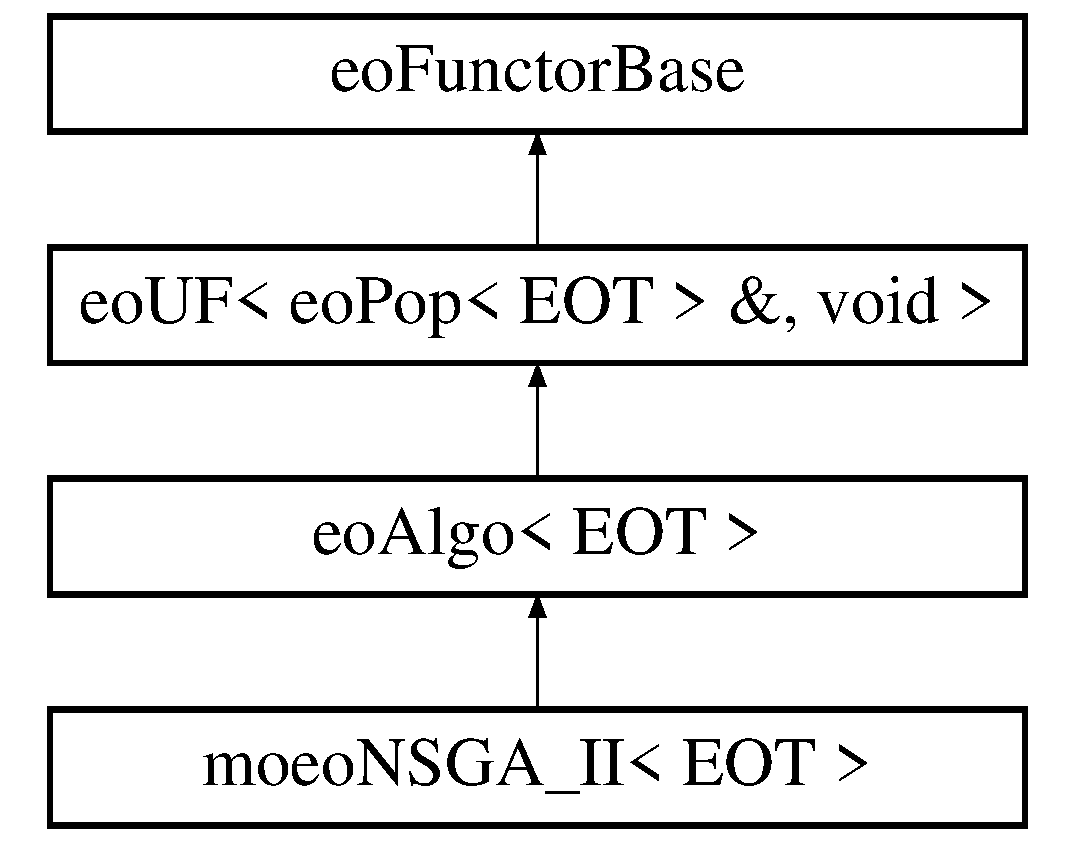
\includegraphics[height=4cm]{classmoeoNSGA__II}
\end{center}
\end{figure}
\subsection*{Public Member Functions}
\begin{CompactItemize}
\item 
{\bf moeo\-NSGA\_\-II} (unsigned \_\-max\_\-gen, {\bf eo\-Eval\-Func}$<$ EOT $>$ \&\_\-eval, {\bf eo\-Gen\-Op}$<$ EOT $>$ \&\_\-op)
\begin{CompactList}\small\item\em This constructor builds the algorithm as descibed in the paper. \item\end{CompactList}\item 
{\bf moeo\-NSGA\_\-II} (unsigned \_\-max\_\-gen, {\bf eo\-Eval\-Func}$<$ EOT $>$ \&\_\-eval, {\bf eo\-Quad\-Op}$<$ EOT $>$ \&crossover, double p\-Cross, {\bf eo\-Mon\-Op}$<$ EOT $>$ \&mutation, double p\-Mut)\label{classmoeoNSGA__II_37109beabe74b0fecb2f3f899ef573d7}

\begin{CompactList}\small\item\em Ctor taking \_\-max\_\-gen, crossover and mutation. \item\end{CompactList}\item 
{\bf moeo\-NSGA\_\-II} ({\bf eo\-Continue}$<$ EOT $>$ \&\_\-continuator, {\bf eo\-Eval\-Func}$<$ EOT $>$ \&\_\-eval, {\bf eo\-Gen\-Op}$<$ EOT $>$ \&\_\-op)\label{classmoeoNSGA__II_29ae86b4254ba6e5263c159df812fb7e}

\begin{CompactList}\small\item\em Ctor taking a continuator instead of \_\-gen\_\-max. \item\end{CompactList}\item 
virtual void {\bf operator()} ({\bf eo\-Pop}$<$ EOT $>$ \&\_\-pop)\label{classmoeoNSGA__II_a9a94b2ee67038b81cdba0fd005350d0}

\begin{CompactList}\small\item\em Apply a few generation of evolution to the population. \item\end{CompactList}\end{CompactItemize}
\subsection*{Protected Attributes}
\begin{CompactItemize}
\item 
{\bf eo\-Continue}$<$ EOT $>$ \& {\bf continuator}\label{classmoeoNSGA__II_22ba11ba501fb7cf3423d9b777294998}

\item 
{\bf eo\-Eval\-Func}$<$ EOT $>$ \& {\bf eval}\label{classmoeoNSGA__II_6b90df8b9890035788a4d4a3f0c26742}

\item 
{\bf eo\-Pop\-Loop\-Eval}$<$ EOT $>$ {\bf loop\-Eval}\label{classmoeoNSGA__II_72fd9c6e70e9ee19db82a6894cafc60b}

\item 
{\bf eo\-Pop\-Eval\-Func}$<$ EOT $>$ \& {\bf pop\-Eval}\label{classmoeoNSGA__II_c1975957e19a164fde96ed7b5ce90ba4}

\item 
{\bf moeo\-NDSorting\_\-II}$<$ EOT $>$ {\bf sorting}\label{classmoeoNSGA__II_1aa7de4992f6c0f1c3a093aca735874c}

\begin{CompactList}\small\item\em NSGAII sorting. \item\end{CompactList}\item 
{\bf eo\-Det\-Tournament\-Worth\-Select}$<$ EOT $>$ {\bf select\-One}\label{classmoeoNSGA__II_add129e06168846b7e405ddd25d70c4d}

\begin{CompactList}\small\item\em Binary tournament selection. \item\end{CompactList}\item 
{\bf moeo\-Elitist\-Replacement}$<$ EOT $>$ {\bf replace}\label{classmoeoNSGA__II_c75535b7a47c26d8a66c1f227d33a3af}

\begin{CompactList}\small\item\em Elitist replacement. \item\end{CompactList}\item 
{\bf eo\-General\-Breeder}$<$ EOT $>$ {\bf gen\-Breed}\label{classmoeoNSGA__II_febee845341b96dba1cdfc18640d4960}

\item 
{\bf eo\-Breed}$<$ EOT $>$ \& {\bf breed}\label{classmoeoNSGA__II_f0dc0665ea743729e6284d812192acfc}

\end{CompactItemize}


\subsection{Detailed Description}
\subsubsection*{template$<$class EOT$>$ class moeo\-NSGA\_\-II$<$ EOT $>$}





Definition at line 31 of file moeo\-NSGA\_\-II.h.

\subsection{Constructor \& Destructor Documentation}
\index{moeoNSGA_II@{moeo\-NSGA\_\-II}!moeoNSGA_II@{moeoNSGA\_\-II}}
\index{moeoNSGA_II@{moeoNSGA\_\-II}!moeoNSGA_II@{moeo\-NSGA\_\-II}}
\subsubsection{\setlength{\rightskip}{0pt plus 5cm}template$<$class EOT$>$ {\bf moeo\-NSGA\_\-II}$<$ EOT $>$::{\bf moeo\-NSGA\_\-II} (unsigned {\em \_\-max\_\-gen}, {\bf eo\-Eval\-Func}$<$ EOT $>$ \& {\em \_\-eval}, {\bf eo\-Gen\-Op}$<$ EOT $>$ \& {\em \_\-op})\hspace{0.3cm}{\tt  [inline]}}\label{classmoeoNSGA__II_bdbf13431487a83afdfd4f527f99ebcf}


This constructor builds the algorithm as descibed in the paper. 

Deb, K., S. Agrawal, A. Pratap, and T. Meyarivan, A fast elitist non-dominated sorting genetic algorithm for multi-objective optimization: NSGA-II. In IEEE Transactions on Evolutionary Computation, Vol. 6, No 2, pp 182-197, April 2002. \begin{Desc}
\item[Parameters:]
\begin{description}
\item[{\em \_\-max\_\-gen}]number of generations before stopping \item[{\em \_\-eval}]evaluation function \item[{\em \_\-op}]variation operator \end{description}
\end{Desc}


Definition at line 46 of file moeo\-NSGA\_\-II.h.

The documentation for this class was generated from the following file:\begin{CompactItemize}
\item 
moeo\-NSGA\_\-II.h\end{CompactItemize}
